%! Author = adnansiddiquei
%! Date = 13/12/2023

\subsection{Q3 - Dataset C}\label{subsec:dataset-c}
    \begin{figure}
    \centering
    \begin{subfigure}{0.9\textwidth}
        \centering
        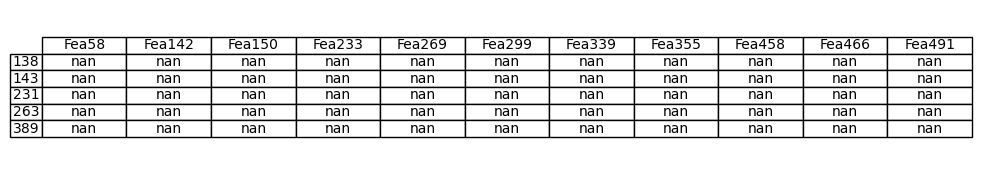
\includegraphics[width=1\textwidth]{./figures/q3a}
        \caption{The samples and features with missing data.}
        \label{fig:q3a}
    \end{subfigure}%
    \hfill
    \begin{subfigure}{0.9\textwidth}
        \centering
        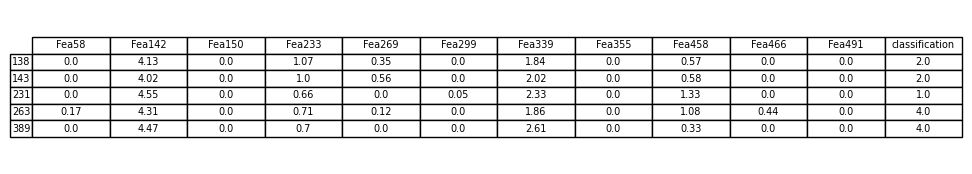
\includegraphics[width=1\textwidth]{./figures/q3c_1}
        \caption{The imputed data.}
        \label{fig:q3c}
    \end{subfigure}
    \caption{Samples and features with missing data, for the \inlinecode{C_MissingData.csv} dataset.}
    \label{fig:q3ac}
    \end{figure}

    Fig\eqref{fig:q3a} shows all the features that have missing values, and all the samples which are missing
    those features.
    There are a few ways to handle missing data.
    A straightforward method is static imputation where every sample missing a given feature, is imputed with the same
    value for that feature, such as the mean of that feature.
    This is computationally inexpensive but can reduce the variance in the dataset and introduce bias if there are many
    missing values.
    Another method is model based imputation where an applicable model is chosen to estimate the value of the missing
    feature for each sample.
    An example is the K Nearest Neighbours approach, where a sample missing a feature is imputed with the mean of the
    K nearest neighbours.
    This can reduce the bias introduced and leave the variance unaffected, but is heavily dependent on the correct
    choice of model.
    Multiple imputation is where the missing data is imputed using a probabilistic model mutliple times, to create
    multiple datasets.
    The multiple imputed values can then either be averaged or the multiple datasets can then be individually analysed,
    Multiple imputation helps capture the uncertainty in what the missing data is, which is useful in the case that
    there is a large amount of missing data.

    Fig\eqref{fig:q3c} shows the imputed data, with aforementioned KNN approach using $k=5$, and also by first splitting
    samples with missing data into their 3 separate classes before applying KNN.
    This model was chosen because the data is known to be a classification dataset and as such, would lead to the best
    imputation as nearby data would most likely resemble what the missing data would be.

    \begin{figure}[htb]
    \centering
    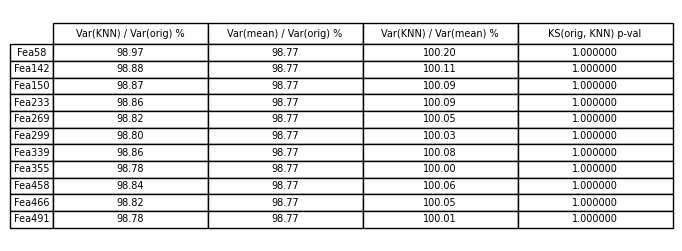
\includegraphics[width=0.9\textwidth]{./figures/q3c_2}
    \caption{A comparison of the variances of each feature after imputation. Column 1 shows the variance of each feature
        after KNN impuration, as a percentage of the original dataset. Column 2 shows this for mean imputation.
        Column 3 compares column 1 against column 2. Column 4 shows the p-value of the Kolmogorov-Smirnov test comparing
        the original dataset to the KNN imputed dataset.}
    \label{fig:q3c_2}
    \end{figure}

    The imputed data does not change the distributions of the features by any statistically significant amount.
    Fig\eqref{fig:q3c_2} shows how the variances of the KNN imputated data compares to the original dataset and a mean
    imputed version of the dataset.
    This indicates that the KNN imputation retains more of the original variance in the dataset compared to a static
    mean imputation.
    Likewise, the Kolmogorov-Smirnov (KS) test was used to compare the distributions of the original dataset and the KNN
    imputed dataset, and the p-value of this test for each feature indicates that KNN imputation did not affect the
    original distributions of the features by any significant amount.
